\section*{Aufgabe 3}

\subsection*{a)}
Sei $K_2$ definiert als $K_2=(Q_2, \Sigma , \Gamma_2 , \delta_2 , Z_2, q_2, F_2 )$.\\
 Mit $\Gamma_2 = \Gamma_1 \cup {E}$ und
 
 $Q_2 = Q_1 \cup \{ q_0, q_{acc}\}$,
 
 $ Z_2 = E \notin \Gamma_1$,

 $q_2 = q_0$ ,
 
 $q_0,q_{acc} \notin Q_1$ ,
 
 $F_2 = \{ q_{acc} \}$
 
Für $q \in Q_1$ ist $\delta_2 (q,a,z) = \delta_1 (q,a,z) $,

 $\delta_2 (q,\varepsilon ,E) = (q_{acc}, Z_1) $ 

 $\delta_2 (q_0,\varepsilon ,Z_0) = (q_1, E Z_1) $
 
 Wie in :
 
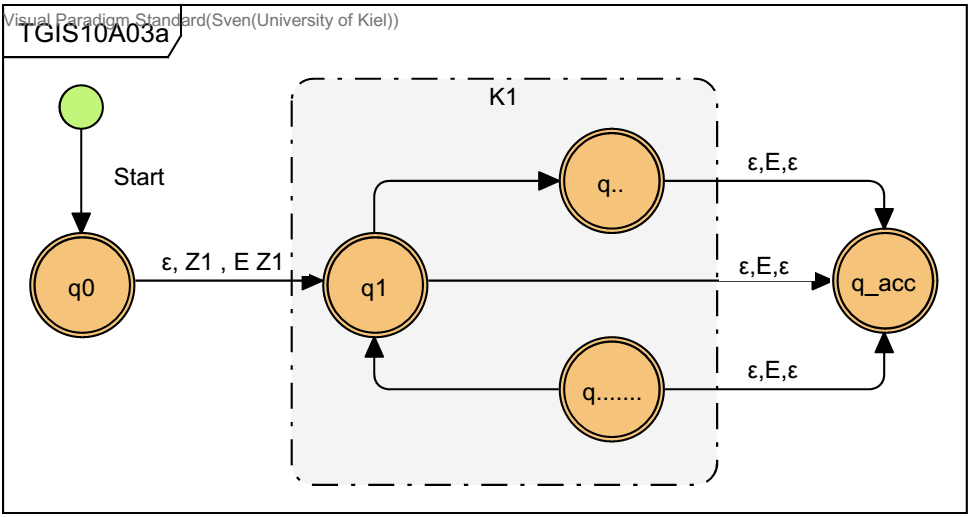
\includegraphics[width=\textwidth]{part/TGIS10A03a}

Idee:

Füge ein Unterstes Element in den Stack und übergehe in $K_1$ wenn ein Zustand keine Eingaben mehr hat und das oberste Element des Stacks das zuerst eingefügte ist gehe in  den akzeptierten zustand.

\newpage

\subsection*{b)}

Sei $K_3 (Q_3,\Sigma, \Gamma_3,\delta_3, Z_3,q_3,F_3)$ KA welcher durch erreichen einer akzeptierenden Zustands akzeptiert.

\subsubsection*{Behauptung}

Es existiert $K_4 = (Q_4,\Sigma,\Gamma_4,\delta_4,Z_4,q_4,\emptyset)$ mit $L(K_3) = L_(K_4)$
und $K_4$ akzeptiert auf leerem Stack.


\subsubsection*{Beweis}

Idee:

Wir fügen eine $K_3$ unbekanntes Symbol $Z_4$ auf dem Stack ein gefolgt von $Z_3$ dann lassen wir $K_3$ laufen,
wenn das Wort eingelesen ist und wir in einem akzeptierenden Zustand von $K_3$ sind leeren wir mit $q_{clear}$ den Stack um zu akzeptieren,
wenn wir nicht in einem akzeptierendm Zustand von $K_3$ sind ist mindestens $Z_4$ noch auf dem Stack und wir leeren den Stack nicht und akzeptieren damit auch nicht.

$q_4 \notin Q_3$

$Q_4 = Q_3 \cup \{ q_{clear},q_4 \}$,

$Z_4 \notin \Gamma_3$,

$\Gamma_4 = \Gamma_3 \cup \{Z_4\}$,

$\forall q \in Q_4 , a \in \Sigma \cup \{\varepsilon\}, k \in \Gamma_4: \delta_4(q,a,k) = $
$\begin{cases}
	\delta_3(q,a,k) \textit{ , für }q \in Q_3 \wedge k \in \Gamma_3 \\
	\{(q_3,Z_4Z_3)\} \textit{ , für } q = q_4 \wedge a = \varepsilon \\
	\{(q_{clear},\varepsilon)\} \textit{ , für } q \in F_3 \cup \{q_{clear}\} \wedge a = \varepsilon \\
	\emptyset \textit{, sonst}
\end{cases}$







